\chapter{Future prospects}
\label{chapter:koopmans_bernardi}

\begin{bf}
  \author{L\'{e}on V. E. Koopmans (Kapteyn Astronomical Institute, University of Groningen),\\ Gianni Bernardi (INAF-IRA \& Rhodes University)}\\
  
Abstract\\
\end{bf}

\noindent This chapter addresses limitations to current 21-cm signal detection instruments, be it related to the instrument, environment, signal-processing or science, and what lies beyond the current horizon for 21-cm science, especially in the 2030s and beyond. We address how to overcome current challenges and drive the field forward, not only approaching a detection of the 21-cm signal but to a full characterisation of its parameter space, in particular, probing an increasingly larger volume of k-modes (spatially and in redshifts). We also will shortly touch upon the kinds of questions that could drive such future endeavours. 

\section{What drives future 21-cm signal experiment?}

The past two decades have witnessed exciting advancements in the field of 21-cm Cosmology. Both theoretically and observationally great progress has been made, although a convincing detection of the 21-cm signal still has to be achieved both for the globally-averaged 21-cm signal as for measuring its spatial fluctuations. We have observed the construction and operation of a vast number of ground-based interferometers (e.g. LOFAR, 21CMA, MWA, NenuFAR, LWA-OVRO, uGMRT, PAPER, refs) and single-element receivers (e.g. EDGES, SARAS, BIGHORNS, PRIZM, SKYHI, refs), covering a wide range in their collecting area, core filling factor, field of view, frequency coverage, observational strategies (e.g. drift scan versus tracking), receiver technology (phased-array versus dishes), etc. Besides these instrument and technology developments driving the field forward, an enormous effort has been afforded to develop much more refined flagging, calibration, imaging, foreground-removal, and 21-cm signal extraction methodologies (refs). These two tracks (instrument and signal processing) have gone hand in hand and have led to steady progression and ever more stringent 21-signal limits (refs). The first confirmed 21-cm signal detection could be well in reach in the coming years. 
%
One of the most exciting and hotly-debated recently developments recently has been the announcement of the detection of the global 21-cm signal by the EDGES collaboration (ref). Although confirmation of this claim is still needed, it shows that astrophysical effects (e.g. bright polarised foregrounds, ionospheric refraction, RFI mitigation) and instrumental challenges (e.g. chromatic leakage, band-pass structure, multi-path propagation, etc.) are controllable over nearly six orders of magnitude, and further improvements are still coming. 
%
These improvements in both instrument design, layout and interferometer versus single receiver technology, also inform each other and hybrid systems are under construction (e.g. LEDA, NenuFAR).
%
Besides, these ongoing experiments and observational programs, the next generation of instruments, of which HERA and the SKA (refs) are the most significant proponents are now underway. Whereas currently instruments are limited to a "statistical detection" of the 21-cm signal power spectra (opposed to the direct detection of the global signal), mostly limited to the EoR due to the increasingly bright foregrounds and stronger ionospheric phase and amplitude errors, these next-generation instruments aim not only to measure the 21-cm signal statistically but image it directly to the mK-level during the EoR but also expand the redshift range to the Cosmic Dawn. This level of sensitivity has required a substantial increase in collecting area and filling factor (by a factor of about ten) over current instruments, thus stepping away for the experimental stage in which many active instruments find themselves. These new or upgraded systems are incorporating many of the lessons learned from past and ongoing efforts.   
%
In this chapter, we will touch upon some of these ongoing and forthcoming developments, although we will not describe each system in extreme detail. Several are already ongoing in terms of extensions of, or improvements to, current instruments. There is also the development of the SKA and HERA coming online fully in the early to later 2020s. Finally we shortly contemplate what lies beyond the current 2030 horizon, in particular instrumentation that can expand the currently envisioned science scope of the next-generation instruments and might require significantly larger collecting areas ($\gg$1~km$^2$) and be space-based (including the lunar environment or surface) to allow one to escape the limits set by the ionosphere and human-made interference at low frequencies. This would allow them to observe the holy grail of high-redshift 21-cm Cosmology, being the era called the {\sl Dark Ages}, which allows a direct probe of questions posed by fundamental physics, inaccessible via any other way than except the 21-cm signal (refs).



\subsection{Limits to current 21-cm signal observations}

As shown in [Koopmans et al. 2015, SKA chapter], core collecting area, its filling factor, and the field of view (FoV) of the instrument primarily drive the statistical sensitivity of an interferometer to the 21-cm signal power spectrum and its imaging capabilities. For direct imaging of the 21-cm signal, or lack thereof inside ionized bubbles, or intensity variations on small scales, the field of view (FoV) is less critical since cosmic variance might not be the driving factor. A limited FoV will increase the sample variance on the large scales, however, in power-spectrum measurements. However, there are many other limits to the instrument as well, besides the sensitivity of measuring the variance of a given 21-cm signal mode in the presence of thermal noise. Some of these limitations we can "control" to some extent and some we can not, and thus have to be avoided (e.g. choose the proper location or controllable set-up of the experiment) or mitigated (i.e. correct for errors in the data in real-time or during post-processing).
%
Below we summarised some of the influences that are currently considered as limiting 21-cm experiments to reach the thermal noise:
%
\noindent {(a) Collecting area:} Although collecting area is one on of the driving factors in sensitivity, it also drives hardware costs especially if the receivers systems being correlated are small and many are needed to reach the required collecting area. Lack of collecting area can also be compensated by increasing the field of view of a system such that more measurements are made of the same $uv$-cells, and more $uv$-cells are sampled, increasing power spectrum sensitivity. This drives up correlator costs, however, so a careful balance needs to be struck between the difference requirements; {(b) Filling factor:} Placing receivers in a smaller core-area, even for fixed collecting area and field of view, increases the sensitivity of the instrument for the simple reason that more independent visibilities are measured per $uv$-cell (i.e. $k$-mode). Since the 21-cm signal of interest is the same per visibility, whereas thermal noise is not, a higher filling factor rapidly increases the power-spectrum sensitivity; {(c) Field of View:} A larger field of view, in general, is related to a smaller receiver element, and more elements to be correlated. For the above-mentioned reasons, this increases the number of independent $uv$-cells and independent 21-cm signal $k-$modes, thereby decreasing the error in the power spectrum; {(d) Frequency Coverage:} Whereas maximizing the frequency coverage from the EoR to the Cosmic Dawn, and even into the Dark Ages (i.e. $z\sim 6 - 200$), would be optimal, in practice this frequency range is  broken up in smaller bands and channels. These bands are also limited in their spectral resolution, and some channels are lost to RFI (e.g. FM band, DAB/DVB; see below) and in some cases not even covered (e.g. below the ionospheric cutoff which limits coverage of the Dark Ages). These instrumental and environmental effects have led to the development of new wide-band receivers (e.g. for SKA and HERA), to the building of instruments in remote locations to avoid RFI, and to the drive to put these instruments in space where they are not affected by the ionosphere (see below); {(e) $UV$-coverage:} This has already been discussed above, and in general is driven by the number of correleated receivers and the density of the core. The limiting factor is often costs of the electronics, the correlators and data storage. However, in some cases longer baselines are necessary to calibrate the instruments in case it is a highly non-redundant array. {(f) (Polarised) Foregrounds:} Foreground emission is a significant complicating factor in a 21-cm signal experiment, not only because they are bright but also because they are polarised in part and have spatial structure. These two effects couple to the ionosphere and the chromatic and polarised nature of the instrument itself even in the absence of any errors, and cause leakage terms from the foregrounds into the 21-cm signal space; {(g) Instrumental effects:} Instrument are not perfect. Receivers need amplifiers to increase the weak electromagnetic signals into a measurable voltage that can be digitized. These low-noise amplifiers are not 100\% stable and can cause both amplitude and phase errors in the visibility data after correlation. When various receivers and amplifiers take part in station-beamforming, these errors become direction-dependent. Secondly, cross-dipole receivers or receivers that measure circular polarisation partly mix Stokes I, Q, U and V power. The reason is that antennae see radiation coming from different projections of the sky, leading to instrumental polarisation. So even if the instrument is nearly perfect, these effects are impossible to avoid. Hence if the sky is partly-polarised, this power mixes in with Stokes I and the 21-cm signal, and causes structure in the 21-cm power spectrum that is undesirable; {(h) Signal processing:} One final difficulty is that inherent to the data processing. Since processing affects the data, via RFI excision, gain calibration, foreground-removal, etc., it can both remove and enhance signals of interest from the data, including the 21-cm signal itself. Processing, if not done very precisely and accurately,  can thus lead to a severe 21-cm signal bias (in general suppression) or an excess variance.  
\\ 

\noindent Besides these limiting factors, mostly instrument-related, two crucial factors are harder to control and will ultimately drive the designs of large-scale future instruments especially at low frequencies towards space.\\

\noindent {\bf (1) Radio Frequency Interference:} Radio frequency interference (RFI) is becoming an increasingly more critical problem for low-frequency telescopes, as human-made signals from, e.g., transmitters, vehicles, mobile phones, satellites, aeroplanes, are now occupying many of the frequency bands previously clean. This increasing RFI occupancy motivates the next generation of instruments to be built in remote desert environments such as the Karroo in South Africa and Western Australia. Going to space is another, albeit expensive option. Just above the Earth, however, any receiver would see a much larger number of transmitters, making the problem worse. Even at a distance of the moon, an RFI suppression of 80dB would be needed to mitigate it to a level that the 21-cm signal from the CD can be observed (ref). In a lunar orbit, the moon would shield the receivers from Earth and also from solar radiation for a fraction of the time, creating an "RFI-free" cone. Recent activity on the lunar far-side, however, might also jeopardize this as well. A receiver on the fare-side of the moon itself might be shielded even more (if far removed from surface activities), although charged particles on the lunar surface might impact such an instrument as well. Despite this, future low-frequency instruments will likely be in space to at least partly mitigate the worsening RFI situation on Earth. \\

\noindent {\bf (2) Ionosphere:} The ionosphere causes both phase and amplitude fluctuations in the received electro signal, which increase in strength toward lower frequencies, and maximal near the plasma frequency cutoff of the ionosphere (around 5-10MHz). The ionosphere has restricted most instruments to frequencies of 30 or even 50MHz and above. The equivalent redshift ranges cover the EoR and CD, but reaching the Dark Ages will be extremely hard, especially in the presence of very bright foreground that couple to the ionosphere. Reaching the Dark Age 21-cm signal, therefore, requires space-based instruments. Even the early Cosmic Dawn around $z\sim 30$ is effectively out of reach because the ionosphere even forthcoming instrument (e.g. HERA and SKA) would cover those frequency bands.\\

\noindent Whereas these technical and environmental reasons will ultimately drive instruments to becomes ever larger and be built on remote places, or even in space, what do we hope such future instrument will tell us?

\subsection{What will drive future 21-cm experiments}

Future experiments will primarily be driven by increasing sensitivity in 21-cm signal regimes already explored, but also by exploring new regimes in redshift and spatial scales. The former has fundamentally driven the development of the high-sensitivity SKA and HERA telescopes, although each with their distinct strategy of increasing sensitivity in various parts of parameter space. These two instruments will be discussed later in the Chapter. Below we will shortly discuss where future instruments can gain the most over current instrument (assuming current instrument will detect the 21-cm signal in the coming years). 

\begin{itemize}
  
\item {\bf Smaller spatial scales:} Most current instruments are limited to rather a small range $k$-modes ($<1$dex) in the power-spectrum where sufficient signal-to-noise can be reached for a detection. The reason is that shorter baselines add coherently for a more extended integration time per $uv$-cell and these are most sensitive to the larger spatial cases (except in the frequency direction). To reach larger $k$-modes or smaller 3D-spatial scales, the instrument in general needs much more collecting area, one of the drivers for SKA-low. HERA tries to reach higher sensitivity by not only increasing collecting area, but also by increasing its field of view, its the filling factor, but at the cost of having redundant $uv$-sampling. The latter makes direct imaging much harder, especially on smaller spatial scales, and possibly might lead to a harder to calibrate the instrument. However, small spatial scales can also be probed via the power spectrum since they are sampled both in the spatial domain as well as in the frequency domain (since frequency corresponds to redshift and hence to comoving distance). SKA aim for minimum redundancy and henced needs 
more collecting area than HERA, but its imaging capabilities are far superior.
    
\item {\bf Direct imaging:} More collecting area and sensitivity on all spatial scales, also opens up an avenue for direct imaging of the 21-cm signal. One of the highest-priority science drivers for the SKA is, therefore, the direct imaging on scales of about ten arcminutes and larger of the 21-cm signal during the EoR. Ionized bubbles can be imaged on even smaller scales since their contrast to the globally-averaged 21-cm signal is very large (about 30 mK versus fluctuations of only a few mK around the bubbles). 

 \item {\bf Higher redshifts:} A third driver of increasing sensitivity is that it enables even higher redshifts to be observed, e.g., those of the Comic Dawn or even the Dark Ages. At higher redshift, the foregrounds are much brighter, increasing the overall system temperature and hence the thermal noise. Integration times therefore rapidly increases with redshift, and nominally only the SKA and HERA can reach the 21-cm signal from the Cosmic Dawn, although the new NenuFAR system might also be sensitive enough. The latter instrument will be short discussed further in this Chapter.
\end{itemize}

\noindent In short, whereas present-day instruments aim for the first detection at several (lower) redshifts and over a limited range of spatial scales, the next generation of instruments will aim to expand these parameter-spaces, but also do direct imaging rather than summarising the signal in some statistics (e.g. the power-spectrum). In Section X, these next-generation instruments will be discussed, where we not only limit ourselves to SKA and HERA but also shortly touch upon extensions to current instruments and their main science drivers.   

\section{Ground-based interferometers}

In this section, we review the status of those 21~cm ground-based interferometers that are under construction, have been upgraded or will be constructed shortly.

\subsection{The Square Kilometre Array -- SKA1\&2}

The Square Kilometre Array (SKA hereafter) is a global effort by a consortium of member-state countries (refs). SKA will consist of at least two entirely different arrays, with SKA-mid to be built in the Karroo desert of South Africa, and SKA-low to be built in Western Australia, each being relatively radio-quiet zones where human-made RFI is limited (although not absent). The site of SKA-mid currently hosts MEERKAT, which will become part of the SKA, and HERA, whereas the site in Western Australia hosts both the MWA and ASKAP. Since only SKA-low will cover the redshifts of the Cosmic Dawn and Epoch of reionization (50-350MHz, or $z=3.1-27.4$), here, we focus only on this instrument. 
%
SKA-low is very similar in design to LOFAR [Mellema et al. 2013; Koopmans et al. 2015], but has some distinct differences as well, primarily related to the receiver design. SKA-low aims to have 512 stations in Phase 1 (denoted by SKA1-low), having 256 log-periodic cross-dipoles receivers that cover the full frequency band and are semi-randomly spread inside a 40\,m diameter circle. The requirement of a high-gain receiver of the full spectral band limits SKA-low's field of view to a cone with an opening angle of about 90 degrees centred on the zenith, but one that maximizes forward gain. The current receiver design also aims for a spectrally smooth band-pass, something rather difficult to realize for a wide-field and wide-band receiver (refs).
%
About 212 stations will be placed inside a central core of about 600\,m, making it about eight times as sensitive in raw collecting areas as LOFAR-HBA, and significantly more than LOFAR-LBA, which currently is unable to reach standard 21-cm signals from the Comic dawn in any reasonable time. The remaining stations will be distributed along three arms that "spiral" outward up to about 65\,km, in the current design.  The long baselines do not go out as far as those of LOFAR but will yield much better $uv$-coverage in short snapshot observations, and enable proper direction-dependent gain calibration of the system. Hence SKA's observational and calibration strategy is very different from that of  HERA (see below). Whereas SKA aims for minimal redundancy to reduce PSF side-lobes and improve imaging and on-sky calibration capabilities, HERA aims for maximum redundancy which enables more rapidly to reach very low thermal-noise errors on a selected set of $uv$-points, but at the cost of its imaging and on-sky calibration capabilities. It remains to be seen which strategy is the most optimal, although one should keep in mind that SKA-low is also built for other science cases, whereas HERA is a pure 21-cm signal experiment and does not have to cater to other science interests. 
%
The sheer collecting area (0.4 \,km$^2$) and instantaneous bandwidth of 300\,MHz (or 150\,MHz when split in dual-beam mode) make SKA1-low the premier instrument in the late 2020s to directly image the 21-cm signal during the EoR from $z\sim 6-12$, covering the 21-cm signal power-spectrum in the range of roughly $ 0.02 < k < 1 $\,cMpc$^{-1}$ (depending on redshift), and push power-spectrum measurements over more limited $k$-ranges deep in to the Cosmic Dawn, as far as $z\sim 20$ or even above. In particular the former will make this a transformational instrument. For example, observing individual ionized structures enables cross-correlations with many other instruments that aim to look for the sources of reionization (e.g. JWST, ALMA, SPICA). Currently, SKA is planned to be operational around 2028, although early science is foreseen several years before that.
%
Finally, ideas for a far-future ($\gg$2030) upgrade to SKA2-low have already been developed [e.g. Koopmans et al. 2015], which nominally foresees an increase in collecting area by a factor of about four. This could not only allow more detailed imaging due to lower thermal noise, but also lower PSF side-lobes, and hence improved image fidelity. Longer baselines also help to remove foreground sources and calibration and enable even higher redshifts and broader ranges of $k-$ modes to be investigated in terms of 21-cm power spectrum measurements.



\subsection{The Hydrogen Epoch of Reionization Array -- HERA}
\begin{figure}[]
\begin{center}
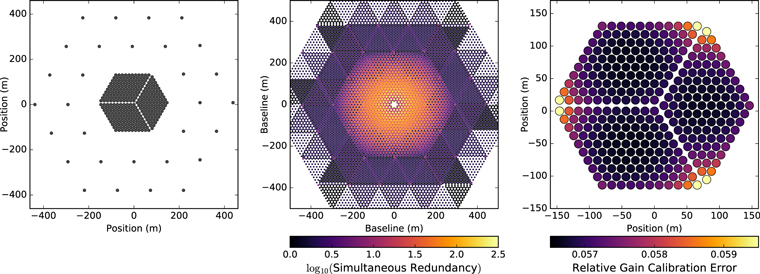
\includegraphics[width=1.\textwidth]{Koopmans_Bernardi/hera_layout}
\end{center}
\caption{The HERA layout (left panel): 320~dishes are located in the hexagonal core and 30 more outrigger dishes are planned to be deployed out to a maximum baselines of $\sim 800$~m to improve angular resolution and imaging capabilities. The core is split in three sectors that are displaced from each other by a fraction of the dish diameter (see \cite{dillon16} for a detailed discussion. The split core provides a significantly improved instantaneous $uv$ coverage (central panel) whilst retaining high redundancy. The right panel shows the expected relative antenna gain errors after using redundant calibration (from \cite{dillon16}).}
\label{fig:fig_hera}
\end{figure}
The Hydrogen Epoch of Reionization Array (HERA, \cite{deboer17}) is an array currently under construction in the Karoo reserve area in South Africa - following the decommissioning of the PAPER experiment (see Chapters~\ref{chapter:bernardi} and 8 in this book for an overview of PAPER). HERA is built following the approach used for PAPER: a highly redundant array to maximize the sensitivity on a number of power spectrum modes measured using the avoidance approach. In order to increase the sensitivity with respect to PAPER, it employs 14~m diameter non steerable dishes that, in the final configuration, will be densely packed in a highly redundant hexagonal array configuration of $\sim 350$~m diameter (see Figure~\ref{fig:fig_hera}). 
HERA main goal is to measure the 21~cm power spectrum in the $6 < z < 12 $ range with high significance in the $0.2 < k < 0.4$~Mpc$^{-1}$ range (\cite{pober14}, providing a full characterization of the evolution of the neutral Hydrogen fraction of the intergalactic medium (Figure~\ref{fig:fig_hera_ion_hist}).
\begin{figure}[]
\begin{center}
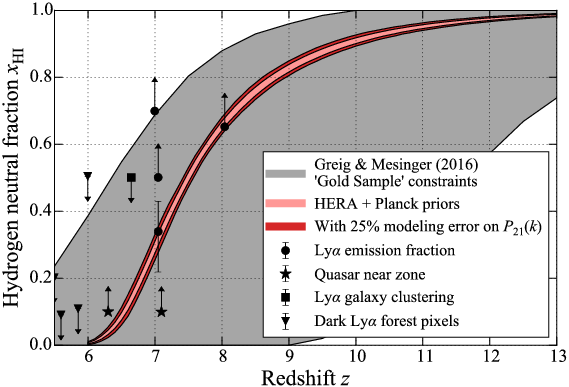
\includegraphics[width=0.6\textwidth]{Koopmans_Bernardi/hera_ion_hist}
\end{center}
\caption{95\% confidence region on the Hydrogen neutral fraction $X_{\rm HI}$ (grey, from \cite{greig17}). The inclusion of HERA measurements leads to a dramatic improvement in the constraints (red and pink areas, \cite{liu16b}). Constraints from other reionization probes are shown as well (see \cite{deboer17} for a detailed description).}
\label{fig:fig_hera_ion_hist}
\end{figure}
%
Given the high redundant configuration, imaging tomography will remain challenging for HERA and likely the goal of a future generation experiment. As foreground modeling and characterization will also be limited because of redundancy and the coarse angular resolution, a significant effort was dedicated to keep the instrumental response from corrupting the intrinsically smooth foreground spectra and to accurately model it (\cite{neben16}, \cite{ewallwice16}, \cite{thyagarajan16}, \cite{patra18}). An alternative approach to redundant calibration is to apply foreground avoidance using closure phase quantities from antenna triads (\cite{thyagarajan18}): closure phase are insensitive to errors in direction independent interferometric calibration and, therefore, directly bypass the requirement of an accurate spectral calibration (see Chapter~\ref{chapter:bernardi} in this book for an overview of calibration of 21~cm observations). A preliminary analysis of HERA closure phases seem to confirm these premises (\cite{carilli18}).
%
HERA is currently under construction, with more than 200 dishes deployed, and 21~cm observations are currently being analyzed. New feeds that extend the sensitivity to the 50-250~MHz range are currently deployed for testing in order to enable observations in the $12 < z < 35$ range (the Cosmic Dawn) and probe the nature of the first luminous sources and their impact on the thermal history of the intergalacic medium.



\subsection{The Large aperture Experiment to detect the Dark Ages -- LEDA}
\label{section:leda_pspec}
\begin{figure}[]
\begin{center}
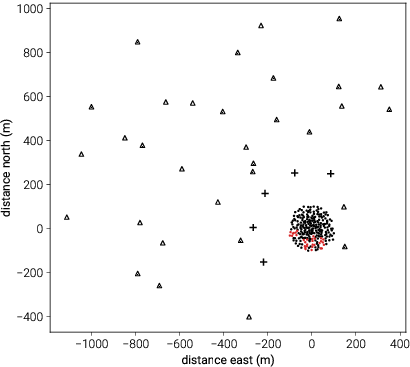
\includegraphics[width=0.6\textwidth]{Koopmans_Bernardi/lwa_layout}
\end{center}
\caption{LEDA antenna layout: the dense core is surrounded by 32 dipoles in order to provide an exceptionally good instantaneous $uv$ coverage (from \cite{eastwood18}).}
\label{fig:fig_leda}
\end{figure}
The Large aperture Experiment to detect the Dark Ages (LEDA, \cite{bernardi15}, \cite{kocz15}) is located at the Owens Valley Radio Observatory, California. It operates in the 30-88~MHz frequency range, corresponding to $15 < z < 46$, seeking to detect the 21~cm signal from the Cosmic Dawn.   
The array layout consists of 251 dipoles pseudo randomly deployed within a 200~m diameter core, 23 dipoles are added out to a maximum 1.5~km baseline (see Figure~\ref{fig:fig_leda}). Five additional outrigger dipoles are custom-equipped to measure the global 21~cm signal via individual custom-built dipoles (see Section~\ref{leda_global}).
%
The very dense core provides exceptional brightness sensitivity and a point spread function with very low sidelobes. The outrigger dipoles improve the angular resolution that helps to identify calibration sources and lower the confusion level. As the dipoles are individually correlated, visibilities have contributions from all-sky emission, particularly from Galactic diffuse emission - given the number of short baselines - and with significant ionospheric-induced refraction and scintillation. Despite these challenges, \cite{eastwood18} generated the first high quality all-sky foreground maps. 
%
The LEDA approach to measure the 21~cm signal can be versatile, allowing to image and subtract foregrounds (\cite{eastwood18}) but also to avoid them (similar to \cite{beardsley16}). \cite{eastwood19} analyzed 20~hours of LEDA data calibrated using a compact source sky model and filtering foregrounds by using their statistical properties in way similar to \cite{dillon14} and \cite{trott16}. They reported an initial $10^8$~mK$^2$ upper limit on the 21~cm power spectrum at $z = 18.4$. Several hundreds of hours of observations have been collected now and will be the focus of future analysis towards the detection of the power spectrum from the Cosmic Dawn and an independent confirmation of the reported detection by \cite{bowman18}.

\subsection{The Low Frequency Array 2.0 -- LOFAR2.0}
\label{section:lofar}

Although LOFAR is already one of the most sensitive arrays for detecting the 21-cm signal during the EoR, its sensitivity is still limited in the redshift/frequency-range of the Cosmic Dawn. This is due to its effective Low-Band Antenna (LBA) collecting area being somewhat limited, and the system temperature at low frequencies being much larger. Furthermore, the LBA dipoles are rather narrow-band, and the gains sharply peak around 60\,MHz, dropping rapidly at frequencies away from the resonance. Similarly, at low frequencies,  ionospheric phase fluctuations increase rapidly making these data harder to calibrate and harder to reach the thermal noise. To mitigate both problems, LOFAR will be upgraded in the coming years. Firstly, half of the 96 dipoles currently in each LBA station is not connected for cost reasons (the cost of an LBA dipole is an order of magnitude lower than the electronics needed to connect it to the overall system), despite being in the field. During the upgrade of LOFAR to LOFAR2 (refs), these 48 LBA-dipoles per station will be connected to the beam-former, effectively doubling the LOFAR-LBA collecting area. This increases LOFAR's sensitivity but also its ability to calibrate on more (fainter) sources, thereby improving ionospheric corrections. Connected to this, currently, only observations can be done in either HBA or LBA mode. LOFAR2 will enable simultaneous observations with the HBA and LBA system, such that the more sensitive HBA system can be used to gain-calibrate the system, including (direction-dependent) ionospheric corrections. Finally, LOFAR2 will in a later stage also enable HBA observations with a dual analogue tile-beam formation, enabling multiple target fields anywhere on the visible sky (not just limited to multiple beams inside the HBA-tile beam, as is currently the case). Each of these improvement enables LOFAR's ability to improve not only the thermal-noise sensitivity to the 21-cm signal but also one's ability to calibrate the system. The first step in this process buy upgrading LOFAR's GPU-based correlator, COBALT, to COBALT2, was recently taken.  

\subsubsection{Amsterdam-ASTRON Radio Transients Facility And Analysis Center -- AARTFAAC}

Whereas LOFAR mainly operates in beam-formed mode, where dipoles or tiles are phased-up in a given direction, the AARTFAAC system (refs) initially build for transient observations currently enables all 576 LBA or HBA dipoles/tiles of the inner 12 stations to be cross-correlated, using two physical correlators, although currently only over a very limited 3.1-MHz bandwidth with 60-kHz resolution. This increase LOFAR's FoV by a factor of about 25 for the HBA system and to all-sky for the LBA system, and increasing the power-spectrum sensitivity by a factor of about 5 or more per unity bandwidth (since both the collecting area and filling factor remain similar and long baselines do not add sensitivity to the 21-cm signal). AARTFAAC is currently already being used to target, for example, the 21-cm signal in the Cosmic dawn as predicted from the EDGES results (refs). An update to AARTWOLF is being planned, where the full correlation of all dipoles/tiles for 24 stations is envisioned over the full LBA and/or HBA bandwidth. This upgrade is closely connected to LOFAR2.0.  

\subsection{New Extension in Nancay Upgrading LOFAR -- NenuFAR}

Another novel array currently in its roll-out and early-science phase is NenuFAR (formerly known as the LOFAR Super Station, LSS). Whereas initially envisioned as an extremely sensitive system between (10)30-85\,MHz in beam-formed mode only, the development of cheap GPU-based correlators for LOFAR (i.e. COBALT) enables NenuFAR in late 2019 to correlate all envisioned 96 mini-arrays, each consisting of 19 LWA-like dipoles, over the full frequency band if high spectral resolution (64 channels of $\sim$3\,kHz each per sub-band of 195\,kHz). The field of view of NenuFAR is about 20 degrees at 60\,MHz, and inside the 400\,m core the filling factor reaches order unity at 35\,MHz, or about $\sim$0.25 at 60\,MHz, which makes it extremely sensitive to low-surface brightness structures. Currently, 56 stations are in place inside a core of about 400\,m diameter, which can be correlated only over 3.1\,MHz of 16 sub-bands (each of 195\,kHz). By late 2019, however, 80 stations will be in place, of which six will be placed further out over an are of about 2.5\,km in diameter. The correlator is already being installed and will also be operational by late 2019. The final goal is to have 96 mini-arrays in place, enabling maximum use of the system. This will make NenuFAR in 2020 one of the most sensitive 21-cm signal arrays in the world, in principle able to reach standard predicted 21-cm signal strengths in the Comic Dawn redshift range (refs). A large observational (key-science) program has started in 2019 to enable this over the coming years.     

\subsection{The Murchison Widefield Array phase II}

Chapters~\ref{chapter:bernardi} and 8 have already described the relevant aspects of the MWA phase II upgrade. Here we emphasize the improved sensitivity to the 21~cm power spectrum due to the addition of the two redundant hexagon near to the core. Figure~\ref{fig:fig_mwa_phaseII_pspec} shows a sensitivity improvement of a factor of four with respect to the phase I and $\sim 10\sigma$ detection of the fiducial 21~cm power spectrum at $k \sim 0.1$~Mpc$^{-1}$. {\bf (GB: Leon, are you ok with this summary?)}
\begin{figure}[]
\begin{center}
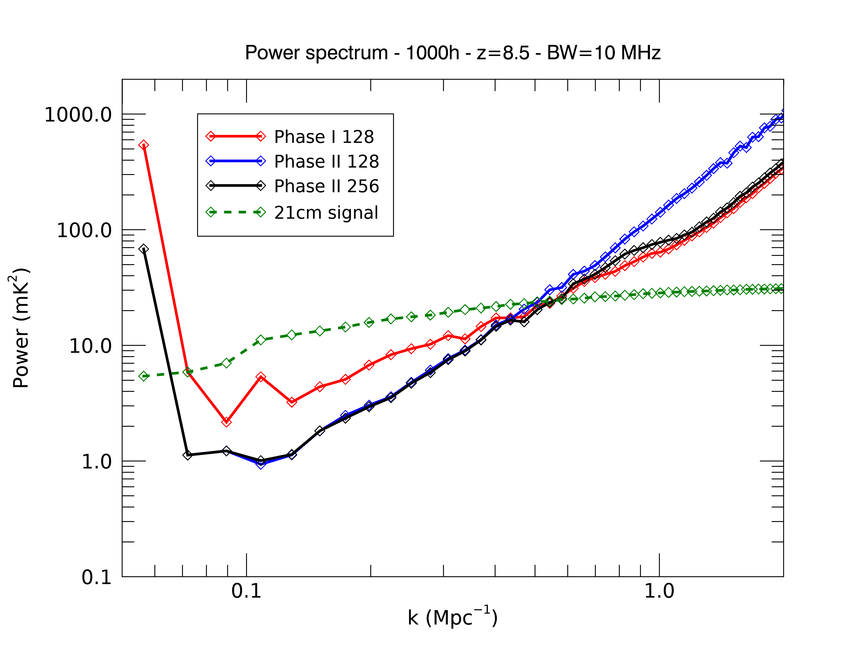
\includegraphics[width=1.\textwidth]{Koopmans_Bernardi/mwa_phaseII_pspec}
\end{center}
\caption{Fiducial 21~cm power spectrum model at $z = 8.5$ with associated noise levels from Phase I and Phase II arrays with a 1000~hour observation. ``Phase II 256" shows the result from a future MWA upgrade where all 256 tiles are correlated simultaneously (from \cite{wayth18}).}
\label{fig:fig_mwa_phaseII_pspec}
\end{figure}




\section{Global Signal Experiments}

In this Section we review the status of the ongoing global signal experiments. 
%(see Chapter~7 for a more detailed discussion about global signal observations).

\subsection{The Experiment to Detect the Global EoR Signature -- EDGES}
%\begin{figure}[]
%\begin{center}
%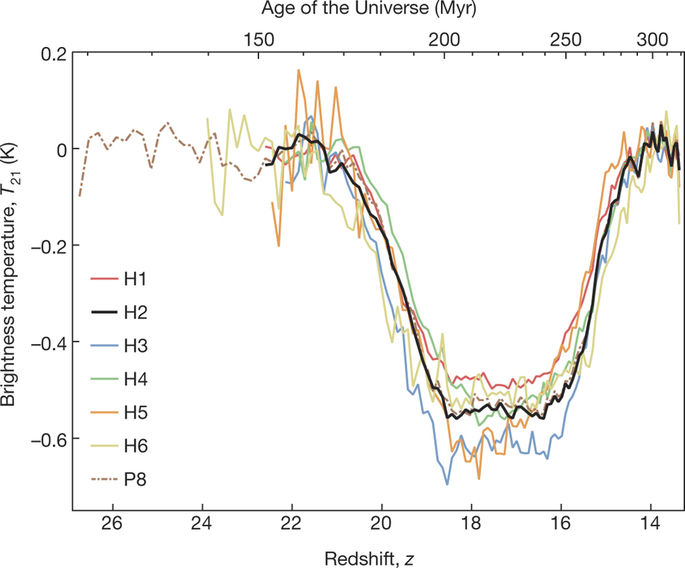
\includegraphics[width=1.\textwidth]{Koopmans_Bernardi/edges_trough}
%\end{center}
%\caption{EDGES}
%\label{fig:fig_edges}
%\end{figure}
The Experiment to Detect the Global EoR Signature (EDGES, \cite{bowman08} currently operates in two frequency bands: the $90-200$~MHz band (high band) in order to constrain the evolution of the neutral fraction throughout reionization, and the $50-100$~MHz band (low band), in order to measure the expected heating of the intergalactic medium from the primordial sources. 
The EDGES experiment has been pioneering techniques to accurately model all the various instrumental components in order to carefully control systematics effects. Observations in the high band have constrained the duration of reionization $\Delta z$ to be longer than $\Delta z >  1$ and started to constrain some properties of the first galaxies (\cite{monsalve17}, \cite{monsalve18}). In the low band, \cite{bowman18} reported the surprising detection of an absorption trough twice as deeper than the most extreme models, posing a serious challenge to its interpretation - assuming it is of cosmological origin. 
In the light of this anomalous signal, the EDGES team is deploying a new dipole antenna tuned in size to simultaneously observe the $60-160$~MHz range (i.e. $\sim 25\%$ smaller than the low band antenna) and confirm the results in the low band. A further upgrade of the EDGES experiment with a more portable antenna that includes the electronics is under consideration for deployment in a quiet radio frequency environment in Oregon, USA.



\subsection{The Large aperture Experiment to detect the Dark Ages -- LEDA}
\label{leda_global}
%\begin{figure}[]
%\begin{center}
%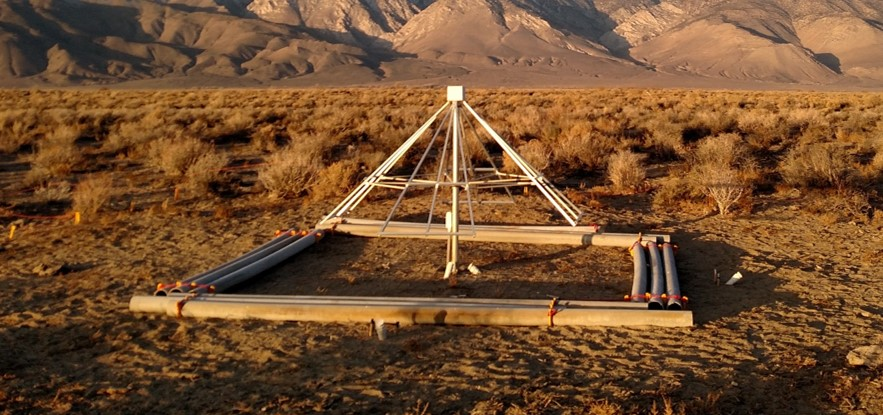
\includegraphics[width=1.\textwidth]{Koopmans_Bernardi/leda_dipole}
%\end{center}
%\caption{LEDA dipole}
%\label{fig:fig_leda_dipole}
%\end{figure}
As mentioned in Section~\ref{section:leda_pspec}, LEDA includes a few custom-equipped dipoles to measure the global signal (\cite{price18}, see also Chapter~7 in this book). Initial observations were used to validate the end-to-end acquisition system and data analysis, leading to a 890~mK upper limit on the global signal amplitude in the $13.2 < z < 27.4$ range at the 95\% confidence level (\cite{bernardi16}). A series of upgrades have been implemented since the early system: filters with a sharper roll-off were installed in order to improve RFI rejection and extend the observing band up to 87.5~MHz in order to validate the results by \cite{bowman18}; the stability of the noise diodes has been improved and a system to measure the ambient temperature at the antenna has been installed. The receiver seems to show the necessary stability to measure the global signal, however, other sources of systematics related to the antenna gain pattern remain lees well known and are the subject of ongoing modeling and investigation.
%
About 100~hours of observations were taken with the upgraded system and are currently being analyzed.
%
%{\bf (GB: this section may be removed if already included in Chapter~7, I cannot see that chapter yet...)}


\subsection{Shaped Antennas to measure the background RAdio Spectrum -- SARAS}

The Shaped Antennas to measure the background RAdio Spectrum (SARAS) represent a progression of radiometers developed over the last decade at the Raman Research Institute and optimized to detect the global 21~cm signal in the $50-200$~MHz range, i.e. in the Cosmic Dawn and Epoch of Reionization.

The SARAS antennas have been designed to provide nearly frequency independent beams and avoid coupling of sky spatial structures into spectral structures in order to preserve the intrinsically smooth foreground spectrum (\cite{sathyanarayana17}).

Initially, SARAS featured a fat-dipole antenna (\cite{patra13}) that was later replaced by a shaped monopole antenna (SARAS~2, \cite{singh18a}). SARAS~2 was deployed in the radio-quiet Timbaktu Collective in Southern India, observing in the $110-200$~MHz. SARAS~2 results disfavoured models with inefficient heating of the intergalactic medium and rapid reionization (\cite{singh17}, \cite{singh18b}). 
A new generation experiment, SARAS~3, exploit a refined design to further reject spurious foreground structures and control over systematics in order to target the 21~cm signal in the $50-100$~MHz band.




\section{Space-based instruments}

Whereas tremendous progress is being made from the ground to detect the globally-averaged and spatially-fluctuating 21-cm signal during the EoR and CD, as discussed earlier, the stability of the system, RFI, the ionosphere, and even multi-path propagation effects, make ground-based observations hard and in some cases, such as a detection of the Dark Ages, even impossible. For this space-based instrument are needed. 
%Are view of some of these can be founds in [Koopmans et al. (2019)]






\subsection{The Dark Ages Polarimetry Pathfinder -- DAPPER}

The Dark Ages Polarimetry Pathfinder (DAPPER, \cite{burns19}) is a space satellite that is intended to observe the global signal from a $\sim 50000$~km lunar orbit, one of the quietest radio frequency environments, with an expected 26~month lifetime. Its goal is to observe the global signal absorption trough that is expected at $17 < \nu < 38$ ($83 > z > 36$), well before the formation of the first luminous sources (see Chapter~2 in this book). In this epoch, the global signal is determined by linear perturbation theory, uncontaminated by complex astrophysical processes. DAPPER is expected to characterize the predicted signal, including any deviation that may be due by the additional cooling reported by \cite{bowman18}. Its strategy includes the use of a polarimeter to measure polarization induced by the anisotropic foregrounds and large antenna beam to aid in the separation of the foregrounds from the isotropic, unpolarized global signal (\cite{nhan17}) and a pattern recognition data analysis that is trained on realisti smulations of observed foregrounds, instrument systematics and the expected global signal (\cite{tauscher18}).
%
DAPPER is one of nine small satellite missions selected by NASA to be further study for a possible launch in the next decade.



\subsection{Discovering the Sky at the Longest Wavelengths -- DSL}

The Discovering the Sky at the Longest Wavelengths (DSL, \cite{chen19}) is a mission concept that explores the possibility to deploy a constellation of micro-satellites circling the Moon on nearly-identical orbits, performing interferometric observations of the sky below 30~MHz, i.e. targeting the Dark Ages. 
Although its sensitivity is insufficient to detect 21~cm fluctuations, its goals will be to accurately image 21~cm foregrounds and to target the 21~cm global using a calibrated single antenna. 

The current DSL concept includes a larger "mother" satellite that leads or trails $5-8$ smaller daughter satellites that carry out radio observations and pass the data to the mother satellite through a microwave link. The mother performs the cross correlation and handles communications with the Earth. 
The DSL project is now undergoing a prototype study.




\subsection{Farside Array for Radio Science Investigations of the Dark ages and Exoplanets -- FARSIDE}

The Farside Array for Radio Science Investigations of the Dark ages and Exoplanets (FARSIDE, \cite{burns19b}) is a mission concept to place an interferometric array on the far side of the Moon, which offers complete isolation from terrestrial radio frequency interference and solar wind, allowing observations at sub-MHz frequencies. The array would consist of 128 dual polarization antenna deployed across a 10~km area by a rover, observing in the $0.1-100$~MHz (basically $z > 13$) range. FARSIDE would also include precision calibration of an individual antenna element via an orbiting beacon in order to attempt the detection of the global 21~cm from the Dark Ages ($50 < z < 100$).

A NASA-funded design study, focused on the instrument, a deployment rover, the lander and base station, delivered an architecture broadly consistent with the requirements for a Probe mission (about 1.3 billion USD).





\subsection{Netherlands-China Low frequency Explorer -- NCLE}

The Netherlands-China Low frequency Explorer (NCLE) is a radio instrument payload on board on the Chines Queqiao relay satellite that orbits behind the Moon. NCLE is designed, built and tested by a Dutch consortium comprised of the Radboud University, ASTRON and ISIS, in close collaboration with the National Astronomical Observatories of the Chinese Academy of Sciences. It is composed of three 5~m long carbon-fibre monopole antenna units that can be switched into dipole mode to observe in the $0.08-80$~MHz range. Its main target is therefore the global 21~cm signal from the Darks Ages and Cosmis Dawn although it will also provide accurate, degree-scale foreground maps below 10~MHz and provide an extensive characterization of the radio frequency interference environment in the lunar far side.

The Queqiao satellite was launched on May 21st, 2018, and is currently behind the Moon, in the Earth-Moon second Lagrange point. NCLE is currently being commissioned, with first observations starting before the end of 2019.


 

\section{The far future of 21-cm cosmology}

The 21-cm signal instruments and experiments described in this book and chapter often have continuously operated already for close to decade (e.g. EDGES, LOFAR, MWA) and have made tremendous progress, possible being on the verge of a detection or enabling to exclude a wide range of 21-cm signal models, either standard (refs) or "exotic" (refs). Some have already been decommissioned and/or are being upgraded since they are reaching the end of their physical lifetime or are merely reaching the maximum of their capabilities (being thermal-noise or systematic-error limited). Entirely new ground-based instruments are also coming online or are being designed at the moment (e.g. NenuFAR, HERA, SKA) to push boundaries various parameter spaces and which will likely dominate 21-cm signal science in the coming decade or two. {\sl However, what lies beyond these instruments? What is still "left to do" when those future instrument have maximised their science return?} As earlier touched upon, besides pushing the boundaries of parameter space in redshift, spatial scale and signal-to-noise (e.g. imaging versus power-spectra measurements), most ground-based instrument are running or will run against limits due to human-made RFI and ionospheric errors or its transparency at very low frequencies. 

The penultimate 21-cm signal instrument should, therefore, be in space, away from RFI and ionospheric errors, enabling not only extremely precise and accurate measurements of the 21-cm signal covering the redshifts of the EoR and CD, but ultimately make a detection of 21-cm signal from the Dark Ages, and also enable direct imaging of the Cosmic Dawn. The challenges that are facing ground-based instruments are impossible to overcome to reach those objectives. For example, at frequencies corresponding to redshifts of the Dark Ages, any radio signal from the sky is distorted by the ionosphere at a level of order unity, on time-scales of seconds. These effects are also direction-dependent and different over scales of arc-minutes. This makes it impossible to correct for and mixes the extremely bright sky of many (tens of) thousands of kelvin with the mK-level 21-cm signal. It is clear that space will be where any instrument has to be to reach the Dark Ages and image the Cosmic Dawn.

Space itself, however, comes with its own challenges. Foremost, bringing and operating a low-frequency instrument in space is expensive and complex. Making the space technology light-weight and still, durable a space-proof is therefore critical. Secondly, being in space does not imply being free of RFI. For example, being in earth-orbit only exacerbates the RFI problem, since any instrument will be exposed to a far larger are on earth. Even near the moon, but still, in view of the earth, RFI needs to mitigated over eight orders of magnitude to drive it below the 21-cm signal. An optimal location is therefore either in deep space where the earth becomes a faint radio source that can be dealt with using traditional excision techniques, but where the sun remains a source of noise, or the instrument can be placed on the back-side of the moon (e.g. FARSIDE) or in lunar orbit (e.g. DLS, DAPPER), where it will be part-time shielded from both the earth and the sun. Even NCLE being about 60,000\,km behind the moon in L2, is not optimally located. With increasing lunar activity (e.g. landers, orbiters), however, even RFI from the lunar surface or orbit might become an issue of concern at some point in time if not carefully thought through or shielded. Where the lunar orbit will not be affected by an ionosphere, the lunar surface is partly charged due to solar radiation (and cosmic rays reaching its surface) and hence even on the lunar surface effects of a lunar "ionosphere" are not absent. On the other hand, reflections of radio waves from the lunar surface back to any orbiter could lead to multi-path propagation and also need mitigation since the dynamic range of the signal can be as high as $10^8$ for the Dark Ages (a sky of 100,000\,Kelvion versus a signal of order a milli-Kelvin).  

Besides these "environmental" effects (e.g. RFI, ionosphere, multi-path propagation), however, any space-based interferometer should have a collecting area that must far exceed that of, e.g. HERA and the SKA. This requirement is not there for global-signal experiments where signal-to-noise is independent of the size of the instrument (of course placing say a hundred similar instruments in space will reach the desired global signal ten times faster). When measuring spatial fluctuations, on the other hand, what counts are the number of visibilities per spatial or $uv$-resolution element and their thermal noise. This drives instrumentation to more receivers elements that are cross-correlated (measuring more modes) and also to a larger collecting area (measuring each model with a smaller thermal-noise error).  To reach the Dark Ages [Koopmans et al. 2019] the necessary collecting areas will be as large as 10-100\,km$^2$ to overcome the thermal noise from the foregrounds that can be as close as $10^5$\,K. Despite these challenges, the information contained in the 21-cm signal during the Dark Ages and also the early Cosmic Dawn will shed light on fundamental physics as well on the astrophysics of the infant Universe, making these developments worth the effort.     


%\section{A Section}
%
%Lorem ipsum dolor sit amet, consectetur adipiscing elit. Duis eu egestas erat. Maecenas tincidunt lacinia tincidunt. Mauris id lectus nec neque feugiat condimentum vitae at diam. In vel orci nunc, non commodo mauris. Vivamus ipsum enim, vulputate quis pharetra non, molestie quis felis. Vivamus porttitor placerat turpis at accumsan. Nunc tortor velit, faucibus a rhoncus nec, blandit non elit. Nam consectetur lectus eu nisi blandit dapibus rhoncus dui tempus. Mauris fermentum dolor vel ipsum vulputate sit amet ultricies tortor lacinia. Donec ut nibh erat. Morbi nec mi ante. Integer nec vestibulum diam. Donec tincidunt pellentesque quam, ut interdum mauris venenatis condimentum. Nam condimentum, augue in aliquet gravida, neque dui elementum eros, id semper eros purus sed felis. Curabitur in justo sit amet sapien ultrices hendrerit at quis nibh. Quisque iaculis pulvinar tincidunt. 
%\begin{eqnarray}
%C(12) &= &\left[\overrightarrow{\pi}\cdot\overrightarrow{\phi}(x+r)\right] \nonumber \\ 
%&\approx& 1-\mathrm{const}\frac{r^2}{L^2}\int_r^L\frac{x\rmd x}{x^2} + \cdots \nonumber  \\
%&\approx& 1-\mathrm{const}\frac{r^2}{L^2}\ln\frac{x\rmd x}{x^2} + \cdots .\label{brokenlongeqn}
%\end{eqnarray}
%
%Aenean tellus risus, porta sit amet porta vitae, tincidunt ut felis. Class aptent taciti sociosqu ad litora torquent per conubia nostra, per inceptos himenaeos. Vestibulum ante ipsum primis in faucibus orci luctus et ultrices posuere cubilia Curae; Phasellus pulvinar placerat velit auctor egestas. Vivamus euismod fringilla tincidunt. Sed ut magna felis, id sollicitudin nunc. Quisque a dui eu erat consectetur egestas a quis justo. Aenean euismod congue diam, vel posuere urna fermentum sit amet. Lorem ipsum dolor sit amet, consectetur adipiscing elit. Mauris faucibus lacus eget est mollis auctor. Donec at nibh ligula, et posuere massa. Phasellus quis leo diam \cite{diamantaras1996pcn}.
%Donec aliquam blandit risus, eu venenatis ante euismod eu. Curabitur cursus justo id arcu condimentum feugiat. Integer sapien urna, vulputate et adipiscing nec, convallis et justo. Suspendisse in ipsum at felis ornare interdum \cite{tulone2006pts},
%
%\begin{figure}[]
%\begin{center}
%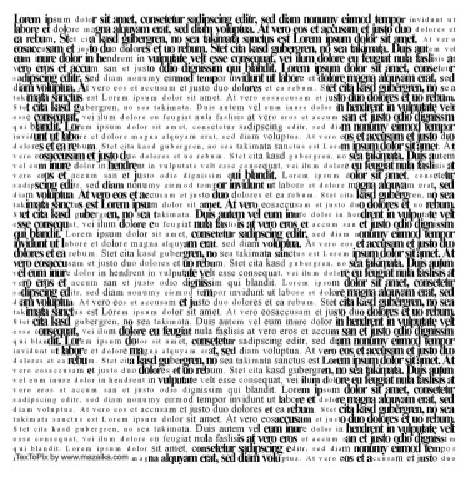
\includegraphics[width=0.5\textwidth]{Koopmans_Bernardi/01x01-eps-converted-to}
%\end{center}
%\caption{This is figure 1 in chapter 1.}
%\end{figure}
%
%\paragraph{Cras adipiscing} sagittis nunc vel luctus. Suspendisse volutpat augue quis erat semper consequat dignissim tellus euismod. Morbi hendrerit, tellus id aliquam iaculis, nibh leo tincidunt eros, vitae varius ligula felis in mi.
%
%\begin{table}
%\caption{Greek Letters.}
%\begin{center}
%\begin{tabular}{llllllll}
%\hline
%$\alpha $  & $ \beta $  & $ \gamma $  & $ \delta $  & $ \epsilon $  & $ \varepsilon $  & $ \zeta $  & $ \eta $ \\
% $ \theta $  &  $ \vartheta $  &  $ \gamma $  &  $ \kappa $  &  $ \lambda $  &  $ \mu $  &  $ \nu $  &  $ \xi $ \\
% $ o $  &  $ \pi $  &  $ \varpi $  &  $ \rho $  &  $ \varrho $  &  $ \sigma $  &  $ \varsigma $  &  $$ \\
% $ \tau $  &  $ \upsilon $  &  $ \phi$ &  $ \varphi $  &  $ \chi $  &  $ \psi $  &  $ \omega$  &  $ $ \\
% &  &  &  &  &  &  & \\
%$ \Gamma $  & $ \Delta $  & $ \Theta $  &  $ \Lambda $  &  $ \Xi $  &  $ \Pi $  &  $ \Sigma $  & $ \Upsilon $ \\
% $ \Phi$ &  $ \Psi $  &  $ \Omega $  &  &  &  &  &\\
%\hline
%\end{tabular}
%\end{center}\end{table}
%
%\begin{figure}[]
%\begin{center}
%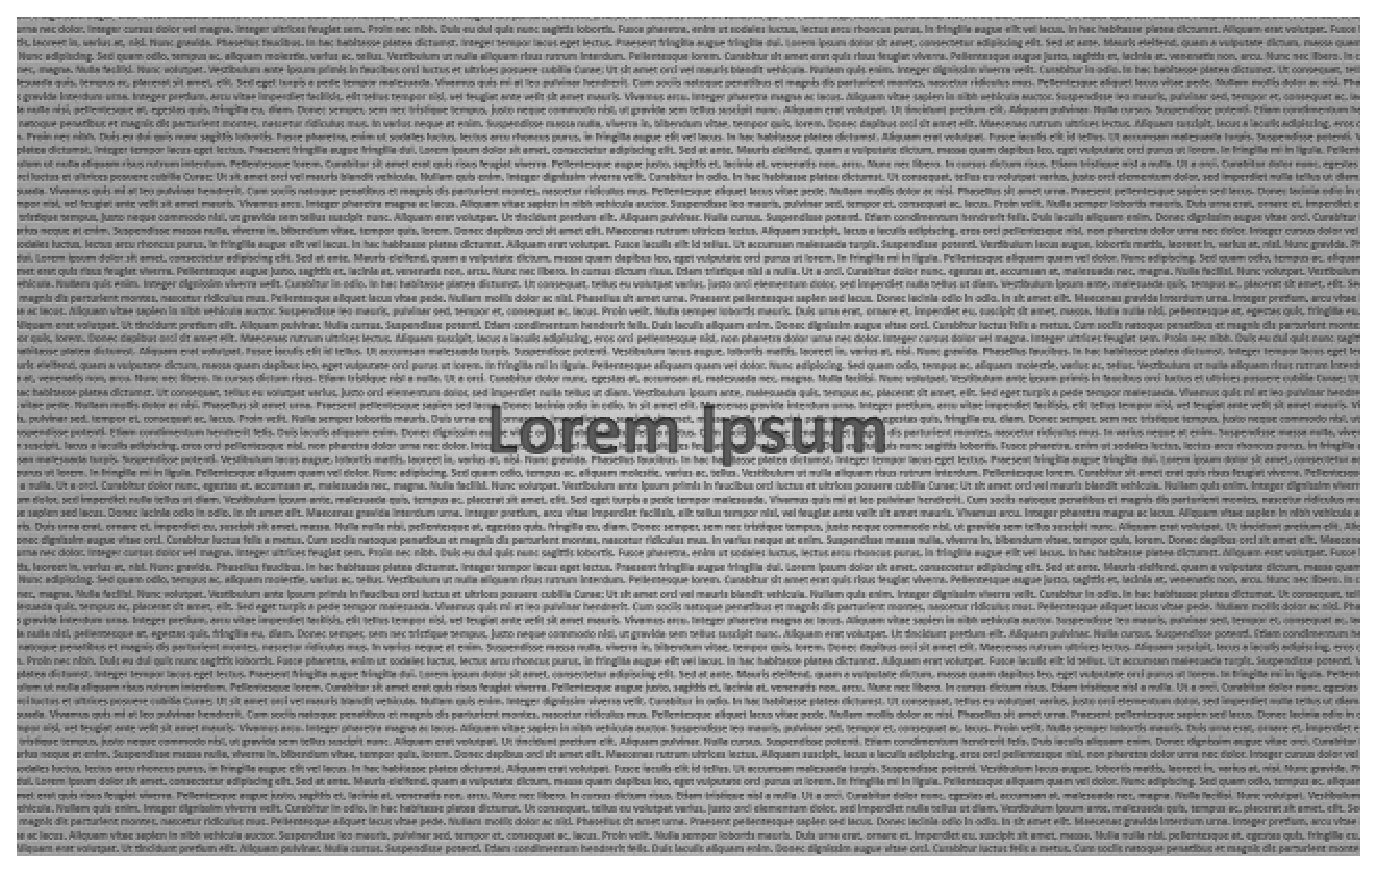
\includegraphics[width=0.6\textwidth]{Koopmans_Bernardi/01x02}
%\end{center}
%\caption{This is figure 2 in chapter 1.}
%\end{figure}


\bibliographystyle{plain}
\bibliography{Koopmans_Bernardi/References}


